\documentclass[11pt,a4paper]{article}

% Packages
\usepackage[margin=1in]{geometry}
\usepackage[utf8]{inputenc}
\usepackage[T1]{fontenc}
\usepackage{amsmath,amssymb}
\usepackage{graphicx}
\usepackage{booktabs}
\usepackage{array}
\usepackage{longtable}
\usepackage{listings}
\usepackage{xcolor}
\usepackage{hyperref}
\usepackage{authblk}
\usepackage{titlesec}
\usepackage{float}

% Hyperref setup
\hypersetup{
    colorlinks=true,
    linkcolor=blue,
    citecolor=blue,
    urlcolor=blue,
    pdfauthor={Firman Hadi, Fauzan Abdullah, Yasser Wahyuddin, L.M. Sabri},
    pdftitle={Spatiotemporal Dynamics of Traffic Congestion Hotspots: A LISA Markov Analysis}
}

% Code listing settings
\lstset{
    backgroundcolor=\color{gray!10},
    basicstyle=\ttfamily\small,
    breaklines=true,
    keywordstyle=\color{blue},
    commentstyle=\color{green!50!black},
    stringstyle=\color{red},
    showstringspaces=false,
    numbers=left,
    numberstyle=\tiny\color{gray},
    frame=single,
    language=Python
}

% Title and authors
\title{\textbf{Spatiotemporal Dynamics of Traffic Congestion Hotspots: A LISA Markov Analysis of Indonesian Cities Using Open-Source Geospatial Tools}}

\author[1]{Firman Hadi\thanks{Corresponding author: firmanhadi21@lecturer.undip.ac.id}}
\author[2]{Fauzan Abdullah}
\author[1]{Yasser Wahyuddin}
\author[1]{L.M. Sabri}

\affil[1]{Department of Geodetic Engineering, Universitas Diponegoro, Semarang, Indonesia}
\affil[2]{Department of Statistics, Faculty of Sciences and Mathematics, Universitas Diponegoro, Semarang, Indonesia}

\date{}

\begin{document}

\maketitle

\begin{abstract}
Understanding the spatiotemporal dynamics of traffic congestion is critical for urban transportation planning. This study applies Local Indicators of Spatial Association (LISA) Markov analysis to examine congestion hotspot persistence and spatial contagion across three Indonesian cities: Jakarta, Bandung, and Semarang. Using the PySAL ecosystem (esda, libpysal, giddy), we analyze 264 million traffic observations across 8 daily time periods. Our findings reveal that smaller cities exhibit higher hotspot persistence, with Semarang showing 18.8\% probability of congestion hotspot retention compared to Jakarta's 6.5\%. Spatial Markov analysis provides evidence of spatial contagion in Bandung ($\chi^2$=8.43, p=0.004) and Semarang ($\chi^2$=6.48, p=0.011), indicating that congestion transitions depend on neighboring segment states. This work demonstrates the effectiveness of open-source geospatial tools for urban traffic analysis and provides insights for targeted congestion mitigation strategies.

\textbf{Keywords:} LISA, Markov chain, spatial contagion, traffic congestion, PySAL, FOSS4G
\end{abstract}

\section{Introduction}

Traffic congestion remains one of the most pressing challenges facing rapidly urbanizing regions across the developing world. In Indonesia, the economic cost of traffic congestion in Jakarta alone is estimated at USD 5 billion annually \cite{worldbank2020}, with significant impacts on productivity, air quality, and quality of life. Beyond economic costs, persistent congestion creates environmental and health burdens through increased vehicle emissions and prolonged travel times.

Traditional traffic analysis approaches often treat congestion as a purely temporal phenomenon, focusing on aggregate metrics like average speeds or volume-to-capacity ratios across entire road networks. However, this perspective overlooks critical spatial dimensions: congestion hotspots are not randomly distributed across urban networks, and their evolution over time exhibits both spatial clustering and temporal persistence. Understanding where congestion emerges, how it spreads between neighboring road segments, and whether certain locations experience chronic versus transient congestion is essential for designing targeted mitigation strategies.

Spatiotemporal analysis methods, particularly those rooted in exploratory spatial data analysis (ESDA), offer powerful tools for uncovering these hidden patterns. Local Indicators of Spatial Association (LISA) can identify statistically significant congestion hotspots and coldspots while accounting for spatial randomness. When combined with Markov chain analysis, these methods reveal temporal transition dynamics: whether segments tend to remain in congested states (persistence) or transition frequently between states (volatility). Furthermore, Spatial Markov analysis tests whether these transitions exhibit spatial contagion---whether a segment's likelihood of becoming congested depends on the congestion state of its neighbors.

The open-source geospatial software (FOSS4G) ecosystem has matured significantly in recent years, with Python-based tools like PySAL providing accessible, reproducible, and extensible frameworks for advanced spatial analysis. Despite this, adoption in operational traffic management contexts remains limited, particularly in developing countries where proprietary software costs pose barriers. This paper demonstrates the effectiveness of FOSS4G tools for analyzing real-world traffic data from three Indonesian cities: Jakarta (14,549 road segments), Bandung (3,069 segments), and Semarang (1,076 segments).

\subsection*{Research Questions}

\begin{enumerate}
    \item How persistent are traffic congestion hotspots across different daily time periods?
    \item Do neighboring road segments influence each other's congestion transitions (spatial contagion)?
    \item How do spatiotemporal congestion dynamics differ across cities of varying sizes and network complexity?
\end{enumerate}

Our contribution is fourfold: (1) We apply LISA Markov analysis to high-resolution traffic data across multiple cities and time periods, (2) We demonstrate the complete workflow using open-source tools (PySAL, GeoPandas, giddy), (3) We release a reproducible data collection and analysis pipeline as an open-source Python package (\texttt{traffic-congestion-pipeline}, available on PyPI), and (4) We provide actionable insights into urban congestion dynamics that can inform infrastructure planning and traffic management policies.

\section{Related Work}

\subsection{Spatial Autocorrelation and LISA}

Spatial autocorrelation---the tendency of nearby locations to exhibit similar values---is a fundamental concept in spatial analysis \cite{tobler1970}. Moran's I statistic \cite{moran1950} provides a global measure of spatial clustering, but local indicators are needed to identify where clusters occur. Anselin \cite{anselin1995} formalized Local Indicators of Spatial Association (LISA), which decompose global spatial autocorrelation into local contributions, enabling identification of statistically significant hotspots (High-High clusters), coldspots (Low-Low), and spatial outliers (High-Low, Low-High).

LISA methods have been widely applied to traffic analysis. Zhang et al.~\cite{zhang2011} identified crash hotspots using Moran's I and LISA in Toronto. Wang et al.~\cite{wang2013} used LISA to detect spatial clustering of traffic incidents in Shanghai. Prasannakumar et al.~\cite{prasannakumar2011} applied spatial autocorrelation to identify accident hotspots in Kerala, India. However, these studies primarily focus on static spatial patterns, treating time as secondary.

\subsection{Markov Chains in Spatial Analysis}

Markov chain models, which describe probabilistic transitions between states, have long been used in geography to analyze land use change \cite{baker1989}, regional income convergence \cite{rey2001}, and urban growth dynamics \cite{batty1976}. The key assumption is that future states depend only on the current state (memoryless property), making transitions tractable to analyze through transition probability matrices.

In transportation research, Markov models have been applied to predict traffic state evolution \cite{li2015}, analyze traffic flow transitions \cite{cheng2012}, and forecast congestion propagation \cite{min2011}. However, these applications rarely incorporate spatial structure explicitly.

\subsection{Spatial Markov Analysis}

Rey \cite{rey2001} introduced the Spatial Markov framework, which conditions transition probabilities on the spatial context---specifically, the state of neighboring locations. This enables testing for spatial contagion: whether transitions are spatially homogeneous or exhibit dependence on neighbors' states. Originally developed for regional income dynamics, Spatial Markov has been applied to urban land transitions \cite{zheng2013} and housing price changes \cite{chegut2015}, but applications to traffic remain scarce.

To our knowledge, this is the first application of LISA Spatial Markov analysis to multi-city traffic congestion data, particularly in a developing country context where infrastructure constraints and rapid urbanization create unique congestion dynamics.

\subsection{Open-Source Geospatial Tools}

The PySAL (Python Spatial Analysis Library) ecosystem has become the de facto standard for spatial econometrics and exploratory spatial analysis in Python \cite{rey2007,rey2021}. The library's modular design separates concerns:
\begin{itemize}
    \item \textbf{libpysal}: Spatial weights and graph construction
    \item \textbf{esda}: Exploratory spatial data analysis (LISA, Moran's I, Getis-Ord)
    \item \textbf{giddy}: Spatial dynamics and Markov analysis
\end{itemize}

Combined with GeoPandas \cite{jordahl2020} for spatial data manipulation and Matplotlib/Seaborn for visualization, this stack provides a complete, open-source workflow for advanced spatial analysis. Our paper showcases these tools on a real-world traffic analysis problem, providing reproducible code that practitioners can adapt to other contexts.

\section{Methodology}

\subsection{Study Area and Data}

We analyze three Indonesian cities representing different urban scales:

\begin{table}[H]
\centering
\caption{Study Cities Characteristics}
\label{tab:cities}
\begin{tabular}{@{}lcccp{5cm}@{}}
\toprule
City & Population & Road Segments & Network Density & Urban Characteristics \\
\midrule
Jakarta & 10.6M & 14,549 & High & Megacity, dense network, complex travel patterns \\
Bandung & 2.5M & 3,069 & Medium & Second-tier city, mountainous terrain \\
Semarang & 1.7M & 1,076 & Low & Coastal city, less congested \\
\bottomrule
\end{tabular}
\end{table}

\textbf{Data Source}: Traffic data were collected from HERE Technologies Traffic API (v8) from March 2025 to February 2026. The API provides the \texttt{jam\_factor} metric (0-10 scale), where 0 represents free-flow conditions and 10 indicates complete standstill. Each road segment's geometry and traffic attributes were retrieved.

\textbf{Temporal Aggregation}: We divided each day into 8 periods to capture diurnal congestion patterns:

\begin{enumerate}
    \item \textbf{Night} (00:00-06:00): Minimal traffic
    \item \textbf{Morning Peak} (06:00-09:00): Commute to work/school
    \item \textbf{Morning Off-Peak} (09:00-11:00): Post-rush hour
    \item \textbf{Lunch Hours} (11:00-13:00): Midday travel
    \item \textbf{Afternoon Off-Peak} (13:00-16:00): Pre-rush hour
    \item \textbf{Evening Peak} (16:00-19:00): Evening commute
    \item \textbf{Evening Off-Peak} (19:00-21:00): Post-work activities
    \item \textbf{Late Night} (21:00-24:00): Nighttime leisure
\end{enumerate}

For each period, we computed the median \texttt{jam\_factor} across all observations within that time window, reducing noise while preserving central tendency.

\textbf{Data Volume}: The complete dataset comprises:
\begin{itemize}
    \item 18,694 unique road segments
    \item 8 time periods per day
    \item 149,552 spatiotemporal observations
    \item $\sim$264 million traffic measurements (aggregated into medians)
\end{itemize}

\subsection{LISA Computation}

For each city-period combination, we computed Local Moran's I statistics using PySAL's \texttt{esda.Moran\_Local} class:

\begin{lstlisting}
from esda import Moran_Local
from libpysal.weights import KNN

# Construct K-Nearest Neighbors spatial weights (k=8)
w = KNN.from_dataframe(gdf, k=8)
w.transform = 'r'  # Row-standardization

# Compute LISA
lisa = Moran_Local(gdf['jam_factor'], w, permutations=999)
\end{lstlisting}

\textbf{Spatial Weights}: We use K-Nearest Neighbors (k=8) rather than distance-based weights because road networks exhibit irregular spacing, and KNN ensures all segments have neighbors regardless of network density.

\textbf{Permutation Testing}: Statistical significance is assessed via 999 random permutations under the null hypothesis of spatial randomness. Segments with pseudo p-values $<$ 0.05 are classified as significant.

\textbf{LISA Categories}: Each segment is assigned to one of five categories:

\begin{itemize}
    \item \textbf{HH (High-High)}: High congestion surrounded by high congestion $\rightarrow$ \textbf{hotspot}
    \item \textbf{LL (Low-Low)}: Low congestion surrounded by low congestion $\rightarrow$ \textbf{coldspot}
    \item \textbf{HL (High-Low)}: High congestion among low neighbors $\rightarrow$ \textbf{spatial outlier}
    \item \textbf{LH (Low-High)}: Low congestion among high neighbors $\rightarrow$ \textbf{spatial outlier}
    \item \textbf{NS (Not Significant)}: No significant spatial pattern
\end{itemize}

\subsection{Classic Markov Analysis}

Given a sequence of LISA categories across the 8 time periods, we model transitions as a first-order Markov chain using \texttt{giddy.markov.Markov}:

\begin{lstlisting}
from giddy.markov import Markov

# y: (n_segments x n_periods) matrix of LISA codes
# Encoded as integers: NS=0, HH=1, LL=2, LH=3, HL=4
m = Markov(y)

# Transition probability matrix P[i,j] = P(period_t+1 = j | period_t = i)
P = m.p

# Steady-state distribution (long-run equilibrium)
steady_state = m.steady_state
\end{lstlisting}

The 5$\times$5 transition matrix $P$ captures the probability that a segment in category $i$ at time $t$ transitions to category $j$ at time $t+1$. Diagonal elements $P_{ii}$ represent \textbf{persistence probabilities}---the likelihood a segment remains in the same state.

\subsection{Spatial Markov Analysis}

To test for spatial contagion, we condition transition probabilities on the \textbf{spatial lag}---the average state of a segment's neighbors. Using \texttt{giddy.markov.Spatial\_Markov}:

\begin{lstlisting}
from giddy.markov import Spatial_Markov

# Spatial weights for conditioning
w = KNN.from_dataframe(gdf, k=8)

# Spatial Markov: transitions conditioned on lag
sm = Spatial_Markov(y, w, permutations=999)

# Chi-squared test for spatial homogeneity
# H0: Transition probabilities are independent of neighbors
chi2 = sm.chi2  # Test statistic for each lag class
\end{lstlisting}

The null hypothesis is that $P(i \to j)$ does not depend on neighbors' states. Rejection (p $<$ 0.05) indicates \textbf{spatial contagion}: transitions are influenced by spatial context.

\subsection{Software and Reproducibility}

All analyses were performed using Python 3.11 with the following key dependencies:

\begin{itemize}
    \item \texttt{geopandas==0.14.3}: Spatial data manipulation
    \item \texttt{esda==2.5.1}: LISA and Moran's I
    \item \texttt{libpysal==4.9.2}: Spatial weights
    \item \texttt{giddy==2.3.5}: Spatial Markov analysis
    \item \texttt{matplotlib==3.8.3}, \texttt{seaborn==0.13.2}: Visualization
\end{itemize}

\textbf{Reproducible Pipeline}: To facilitate replication and extension of this work, we developed \texttt{traffic-congestion-pipeline}, a Python package that automates the complete workflow from data collection to analysis. The package is available on PyPI:

\begin{lstlisting}[language=bash]
pip install traffic-congestion-pipeline
\end{lstlisting}

This package provides command-line tools and Python APIs for:
\begin{itemize}
    \item Multi-provider traffic data collection (HERE, TomTom, Google)
    \item Automated spatial aggregation and temporal binning
    \item LISA computation with configurable spatial weights
    \item Markov chain and Spatial Markov analysis
    \item Publication-ready visualization generation
\end{itemize}

Complete code, analysis scripts, and documentation are available at: \url{https://github.com/firmanhadi21/traffic-analyses}

\section{Results}

Our analysis reveals distinct spatiotemporal congestion dynamics across the three cities, with notable differences in hotspot persistence, transition volatility, and spatial contagion effects.

\subsection{LISA Spatial Clustering Patterns}

\begin{figure}[H]
\centering
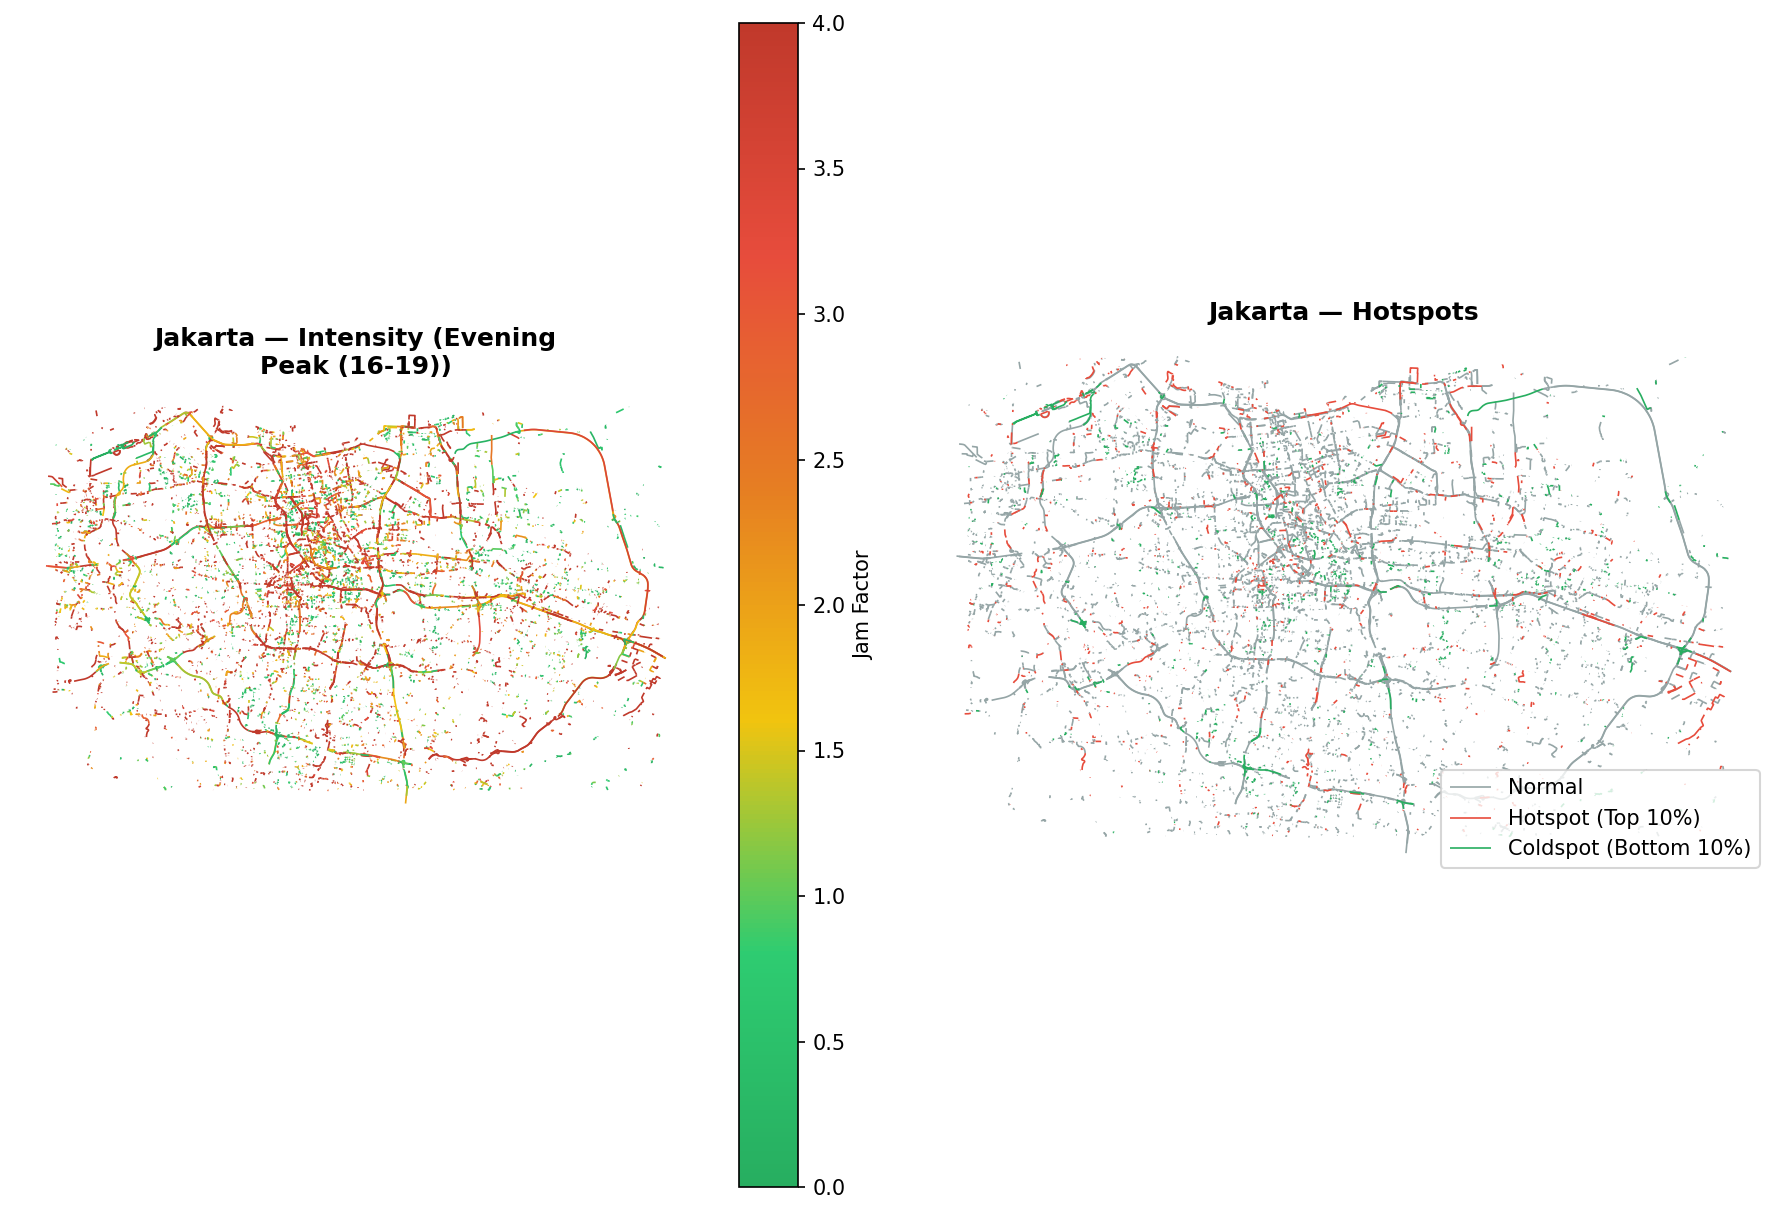
\includegraphics[width=0.32\textwidth]{../figures/jkt_hotspots_evening_peak.png}
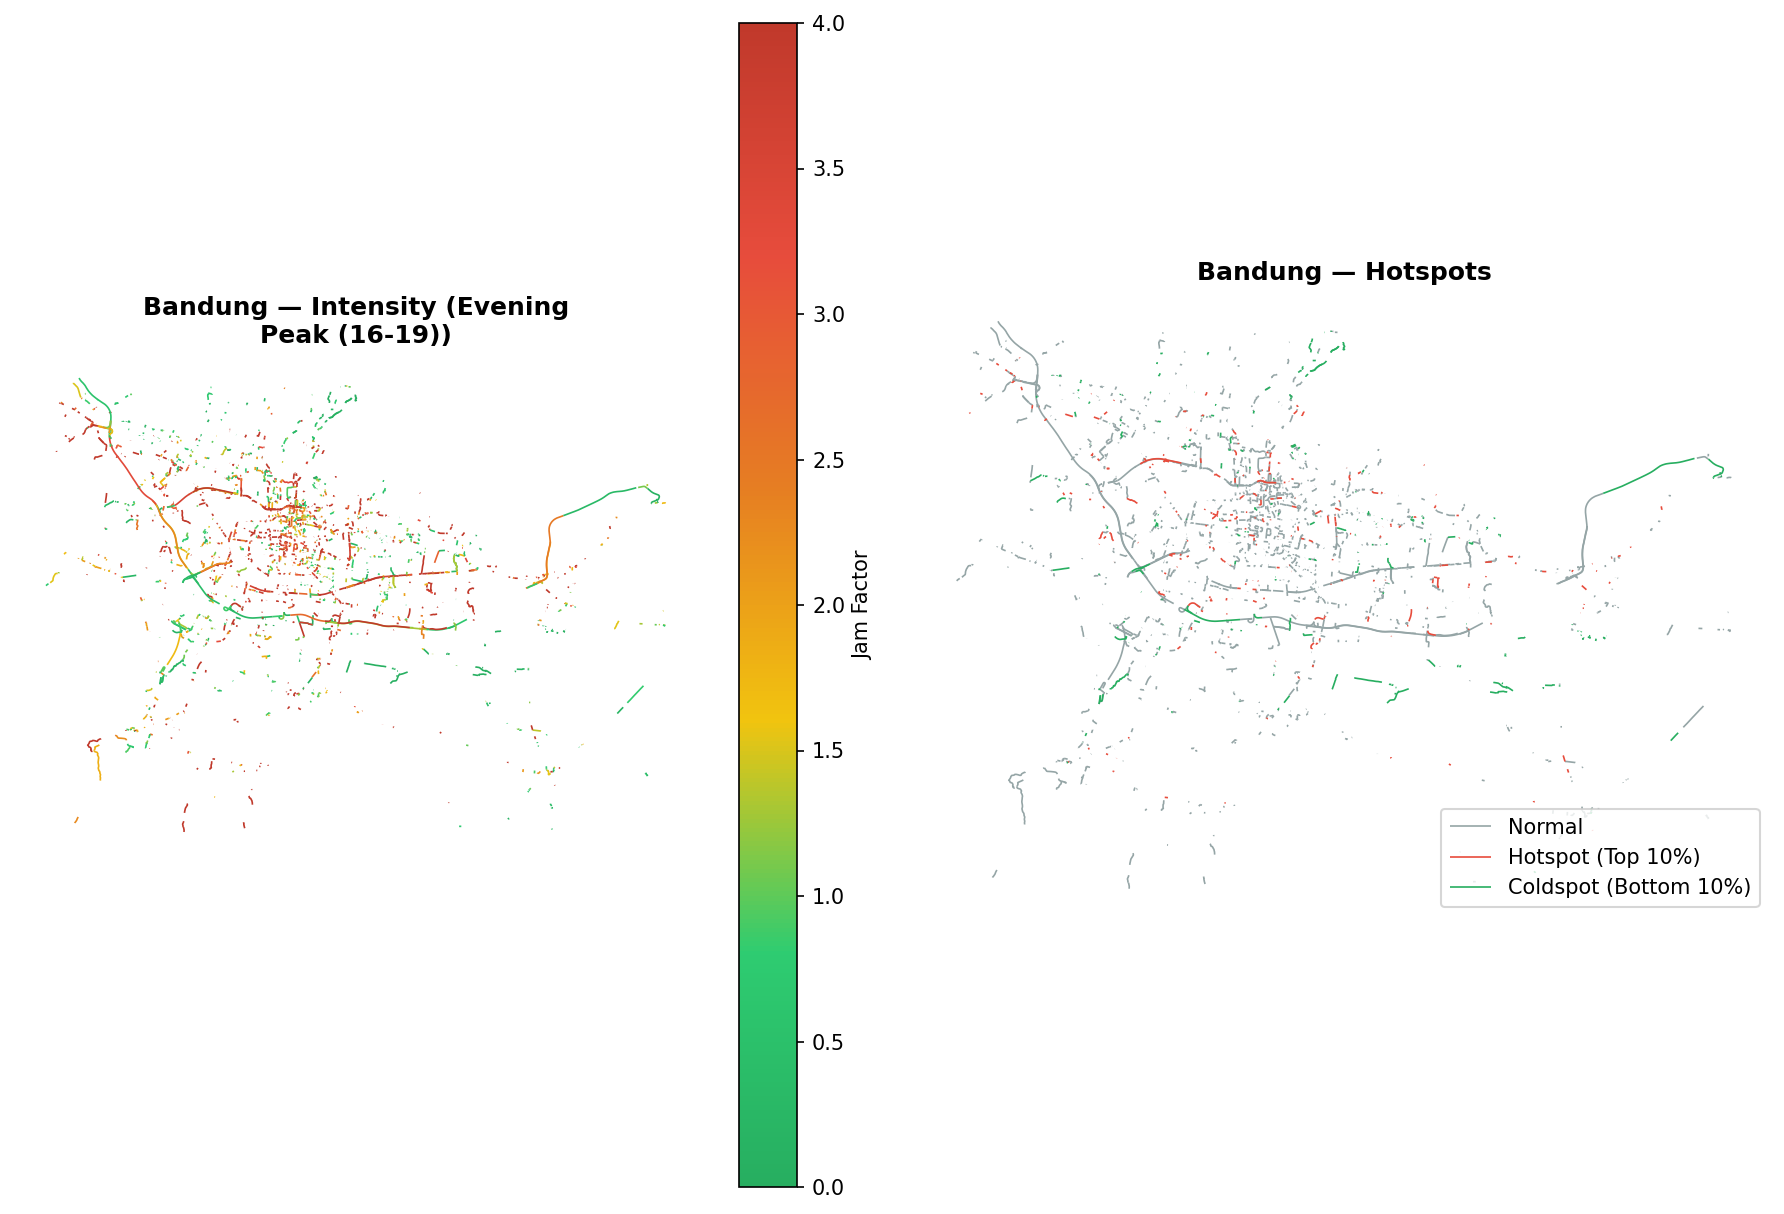
\includegraphics[width=0.32\textwidth]{../figures/bdg_hotspots_evening_peak.png}
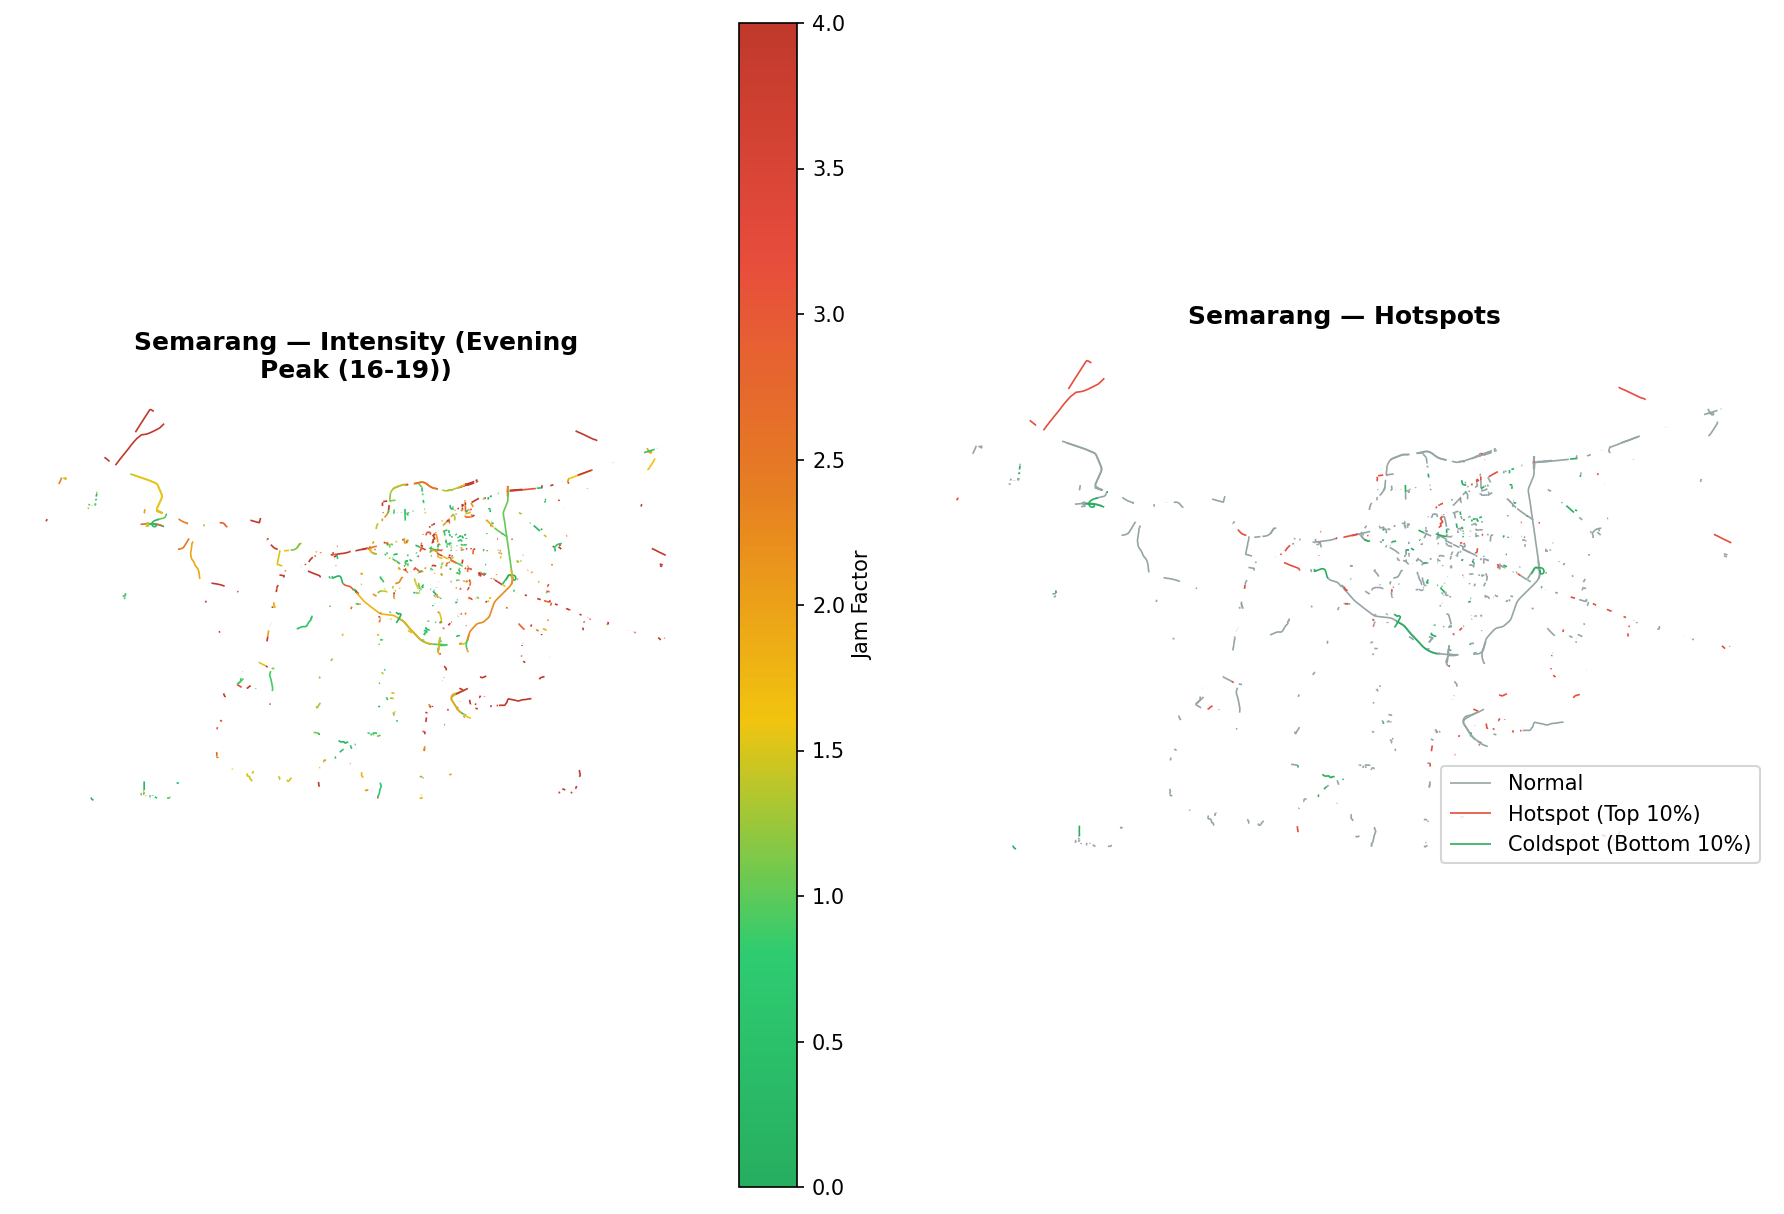
\includegraphics[width=0.32\textwidth]{../figures/smg_hotspots_evening_peak.png}
\caption{LISA cluster maps for evening peak period (16:00-19:00). Left: Jakarta, Center: Bandung, Right: Semarang. Red indicates High-High hotspots (HH), blue shows Low-Low coldspots (LL).}
\label{fig:lisa-maps}
\end{figure}

Figure \ref{fig:lisa-maps} shows representative LISA cluster maps for the evening peak period (16:00-19:00), when congestion is most severe. Across all cities, spatial clustering is evident: congestion hotspots (HH) and coldspots (LL) form coherent spatial regions rather than random dispersions.

\textbf{Jakarta} exhibits the most complex pattern, with multiple disconnected hotspot clusters distributed across the metropolitan area. The highest intensity hotspots appear in central business districts and major arterial bottlenecks. Approximately 16.5\% of segments experienced at least one hotspot designation across the 8 periods, but only 0\% remained consistently classified as HH across all periods---indicating high temporal volatility.

\textbf{Bandung} shows more concentrated hotspot regions, particularly around university districts and commercial centers. The mountainous terrain constrains the road network, creating persistent bottlenecks at key corridors. Here, 14.5\% of segments ever became hotspots.

\textbf{Semarang}, the smallest city, displays the most persistent spatial patterns. Hotspots concentrate along coastal arterials and the central business district, with 9.2\% of segments entering HH state. The lower percentage reflects less severe congestion overall, but those hotspots that do form are more stable.

\subsection{Classic Markov Transition Probabilities}

\begin{figure}[H]
\centering
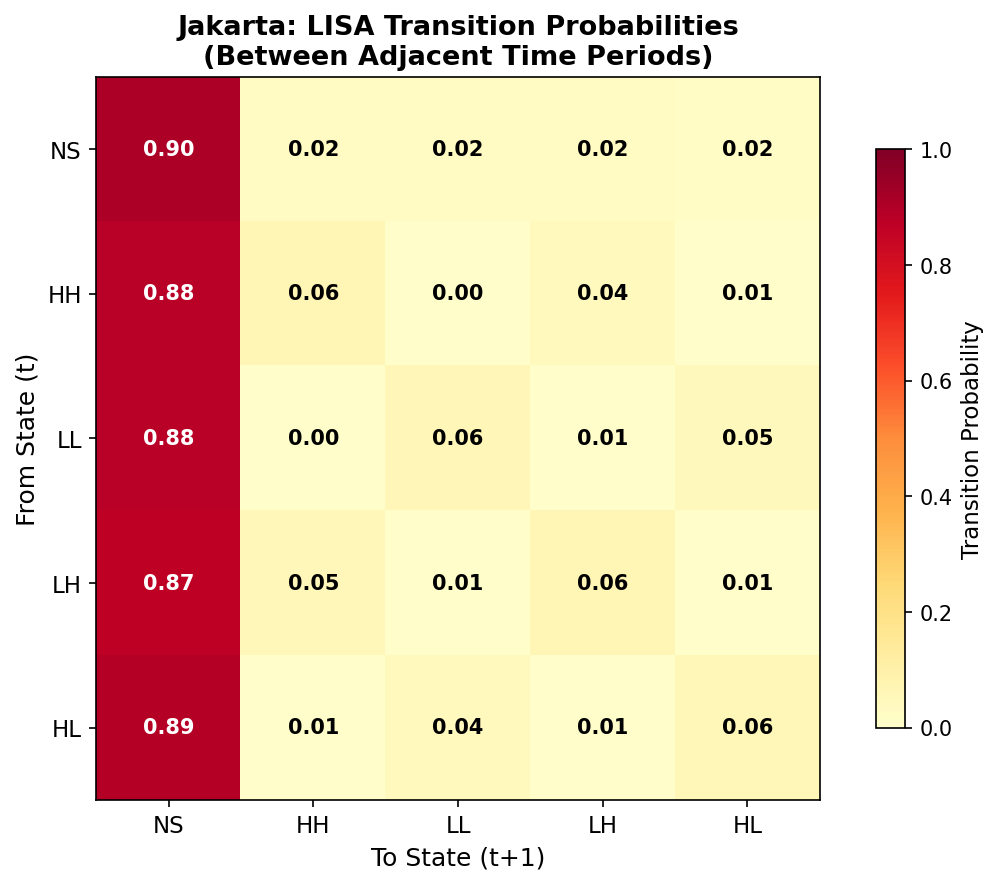
\includegraphics[width=0.32\textwidth]{../figures/markov/jkt_transition_matrix.png}
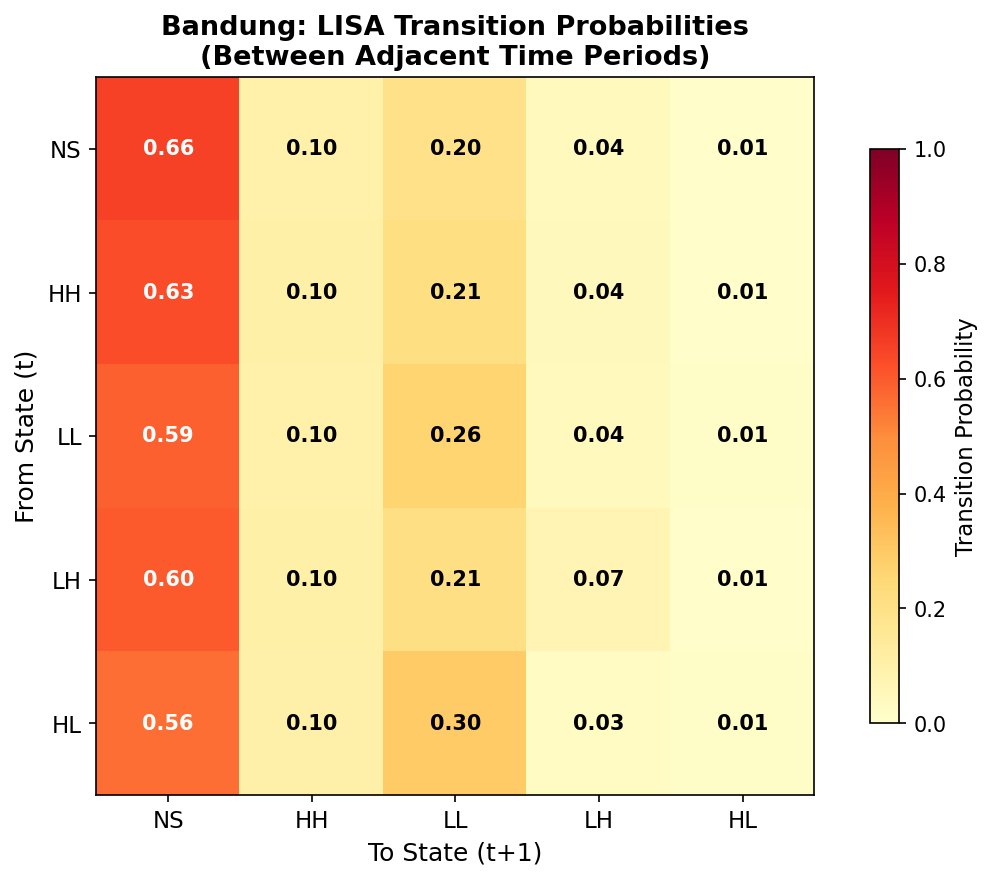
\includegraphics[width=0.32\textwidth]{../figures/markov/bdg_transition_matrix.png}
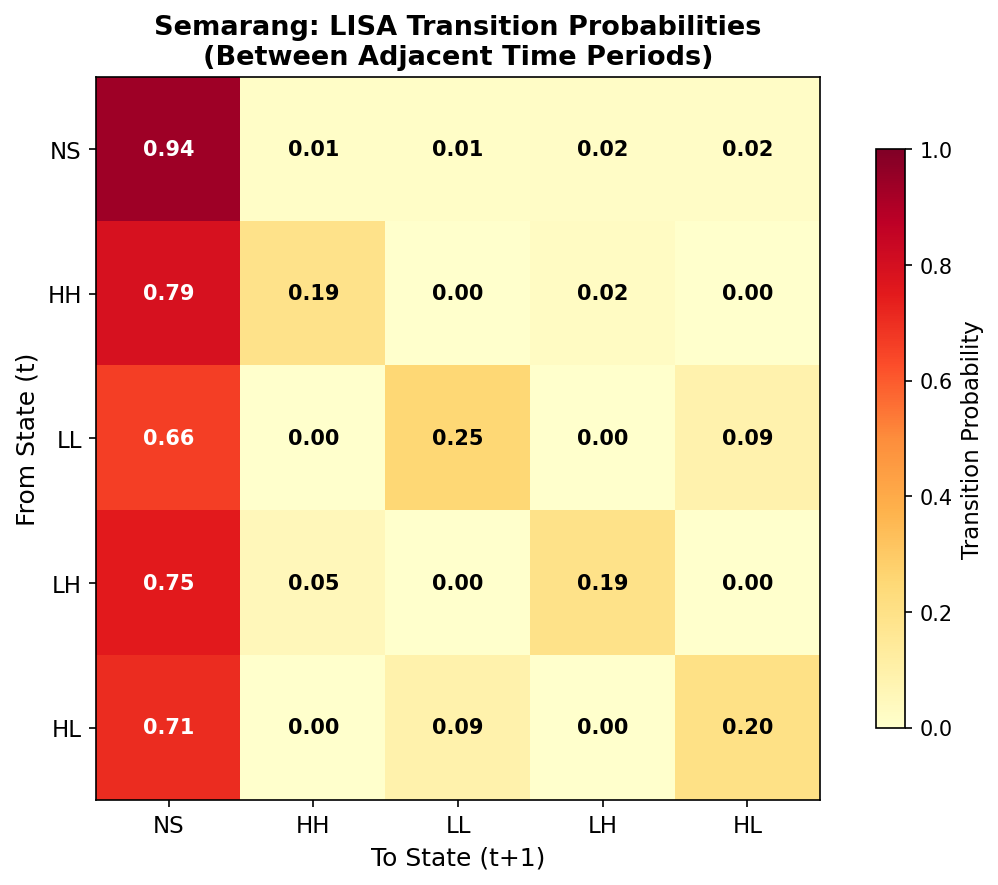
\includegraphics[width=0.32\textwidth]{../figures/markov/smg_transition_matrix.png}
\caption{Transition probability matrices as heatmaps. Left: Jakarta, Center: Bandung, Right: Semarang. Darker colors indicate higher probabilities.}
\label{fig:transition-matrices}
\end{figure}

Tables \ref{tab:jakarta-markov}, \ref{tab:bandung-markov}, and \ref{tab:semarang-markov} present the transition matrices for each city, also visualized as heatmaps in Figure \ref{fig:transition-matrices}. The matrices exhibit strong diagonal dominance: most segments remain in their current LISA category from one period to the next. This temporal inertia is expected---traffic conditions evolve gradually within a day rather than exhibiting abrupt state changes.

\begin{table}[H]
\centering
\caption{Jakarta Transition Probability Matrix}
\label{tab:jakarta-markov}
\begin{tabular}{@{}lccccc@{}}
\toprule
From/To & NS & HH & LL & LH & HL \\
\midrule
NS & \textbf{90.4\%} & 2.4\% & 2.5\% & 2.5\% & 2.3\% \\
HH & 87.9\% & \textbf{6.5\%} & 0.4\% & 4.2\% & 1.0\% \\
LL & 88.1\% & 0.4\% & \textbf{6.1\%} & 0.8\% & 4.7\% \\
LH & 87.0\% & 5.1\% & 0.7\% & \textbf{6.4\%} & 0.8\% \\
HL & 88.7\% & 0.9\% & 4.0\% & 0.6\% & \textbf{5.8\%} \\
\bottomrule
\end{tabular}
\end{table}

\begin{table}[H]
\centering
\caption{Bandung Transition Probability Matrix}
\label{tab:bandung-markov}
\begin{tabular}{@{}lccccc@{}}
\toprule
From/To & NS & HH & LL & LH & HL \\
\midrule
NS & \textbf{90.8\%} & 2.1\% & 2.6\% & 2.3\% & 2.1\% \\
HH & 79.4\% & \textbf{12.0\%} & 0.4\% & 8.2\% & 0.0\% \\
LL & 81.9\% & 0.2\% & \textbf{10.9\%} & 0.5\% & 6.5\% \\
LH & 76.3\% & 9.8\% & 0.2\% & \textbf{13.7\%} & 0.0\% \\
HL & 78.3\% & 0.4\% & 6.2\% & 1.0\% & \textbf{14.1\%} \\
\bottomrule
\end{tabular}
\end{table}

\begin{table}[H]
\centering
\caption{Semarang Transition Probability Matrix}
\label{tab:semarang-markov}
\begin{tabular}{@{}lccccc@{}}
\toprule
From/To & NS & HH & LL & LH & HL \\
\midrule
NS & \textbf{93.6\%} & 1.3\% & 1.5\% & 1.7\% & 1.9\% \\
HH & 78.9\% & \textbf{18.8\%} & 0.0\% & 2.3\% & 0.0\% \\
LL & 66.1\% & 0.0\% & \textbf{25.1\%} & 0.0\% & 8.7\% \\
LH & 75.3\% & 5.3\% & 0.0\% & \textbf{19.3\%} & 0.0\% \\
HL & 70.6\% & 0.0\% & 9.1\% & 0.0\% & \textbf{20.3\%} \\
\bottomrule
\end{tabular}
\end{table}

\textbf{Key Observations:}

\begin{enumerate}
    \item \textbf{Persistence Gradient}: Diagonal probabilities (boldface) increase from Jakarta $\rightarrow$ Bandung $\rightarrow$ Semarang for cluster states (HH, LL, LH, HL). Semarang's P(HH$\rightarrow$HH) = 18.8\% is nearly 3$\times$ higher than Jakarta's 6.5\%.
    
    \item \textbf{Regression to NS}: All cluster states show high probability of transitioning back to NS (not significant). This reflects the temporal nature of congestion: hotspots form during peak hours but dissipate during off-peak periods.
    
    \item \textbf{Asymmetric Transitions}: Hotspots (HH) in Bandung have a notable transition probability to LH (8.2\%), suggesting that as peak periods wane, segments transition from high-among-high to low-among-high---their own congestion clears while neighbors remain congested.
\end{enumerate}

\subsection{Hotspot Persistence Analysis}

\begin{figure}[H]
\centering
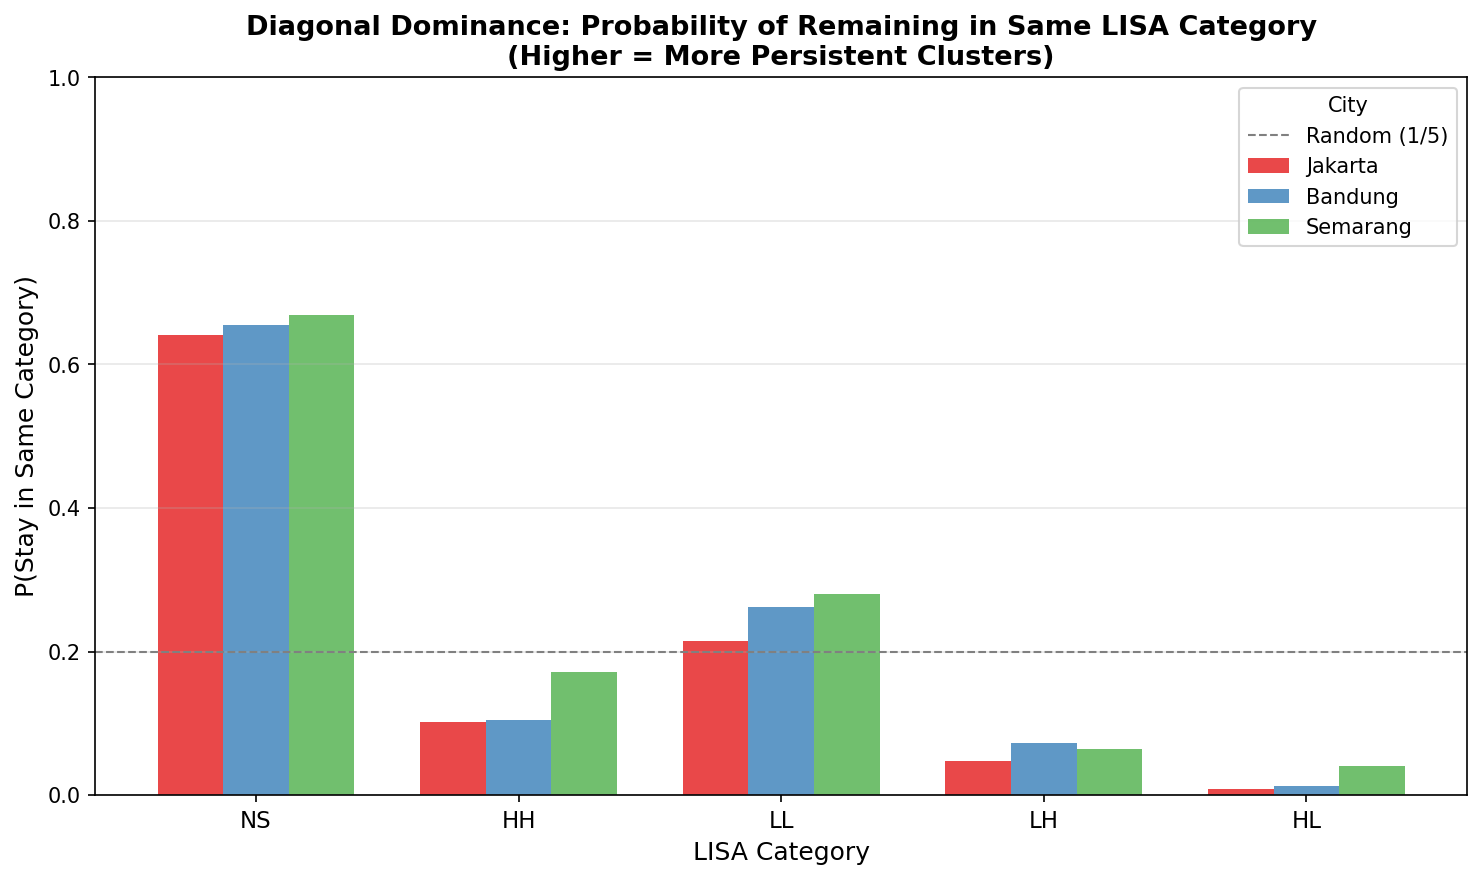
\includegraphics[width=0.85\textwidth]{../figures/markov/diagonal_dominance.png}
\caption{Diagonal dominance (persistence probabilities) comparison across cities for key LISA states.}
\label{fig:persistence}
\end{figure}

Figure \ref{fig:persistence} compares diagonal dominance (persistence probabilities) across cities. We focus on three key states:

\begin{table}[H]
\centering
\caption{Persistence Probabilities Comparison}
\label{tab:persistence}
\begin{tabular}{@{}lccc@{}}
\toprule
City & P(NS$\rightarrow$NS) & P(HH$\rightarrow$HH) & P(LL$\rightarrow$LL) \\
\midrule
Jakarta & 90.4\% & 6.5\% & 6.1\% \\
Bandung & 90.8\% & 12.0\% & 10.9\% \\
Semarang & 93.6\% & 18.8\% & 25.1\% \\
\bottomrule
\end{tabular}
\end{table}

\textbf{Interpretation}: The inverse relationship between city size and cluster persistence suggests that larger, more complex networks exhibit greater congestion volatility. Jakarta's hotspots are short-lived, potentially due to:
\begin{itemize}
    \item More alternative routes enabling traffic redistribution
    \item Dynamic driver behavior responding to real-time information
    \item Greater heterogeneity in trip purposes and timing
\end{itemize}

Conversely, Semarang's high persistence (P(LL$\rightarrow$LL) = 25.1\%) indicates structural constraints: certain segments remain chronically uncongested (e.g., peripheral roads), while hotspots, once formed, are harder to dissolve due to limited network redundancy.

\subsection{Steady-State Distributions}

\begin{figure}[H]
\centering
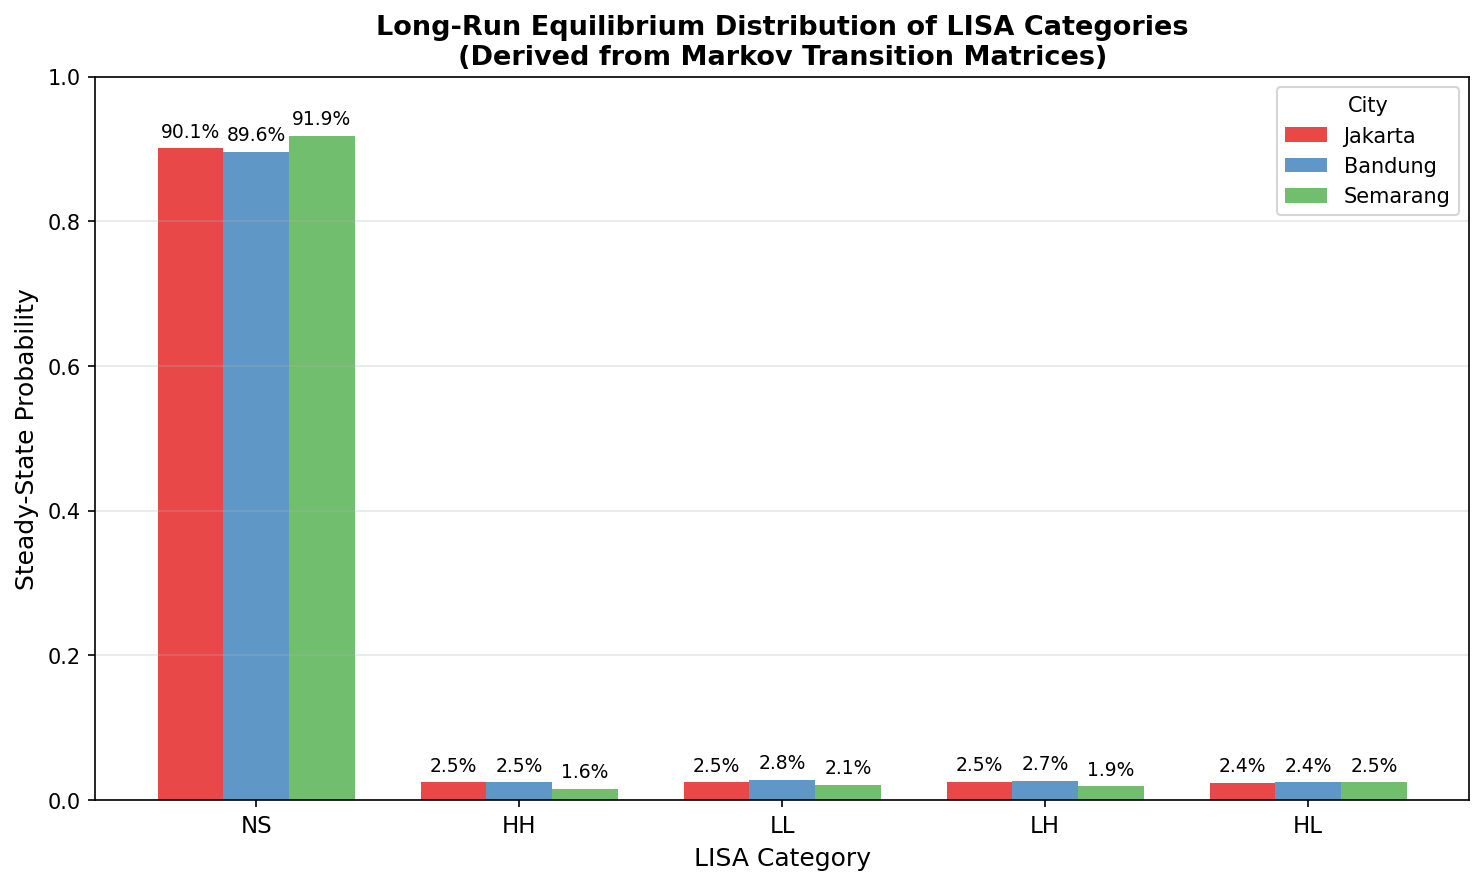
\includegraphics[width=0.75\textwidth]{../figures/markov/steady_state_comparison.png}
\caption{Steady-state distributions across cities showing long-run equilibrium probabilities for each LISA category.}
\label{fig:steady-state}
\end{figure}

All three cities converge to similar long-run equilibrium distributions (Table \ref{tab:steady-state} and Figure \ref{fig:steady-state}):

\begin{table}[H]
\centering
\caption{Steady-State Distributions}
\label{tab:steady-state}
\begin{tabular}{@{}lccc@{}}
\toprule
State & Jakarta & Bandung & Semarang \\
\midrule
NS & 90.1\% & 89.6\% & 91.9\% \\
HH & 2.5\% & 2.5\% & 1.6\% \\
LL & 2.5\% & 2.8\% & 2.1\% \\
LH & 2.5\% & 2.7\% & 1.9\% \\
HL & 2.4\% & 2.4\% & 2.5\% \\
\bottomrule
\end{tabular}
\end{table}

Despite different transition dynamics, all cities stabilize at approximately 90\% NS and 2-3\% in each cluster category. This suggests a universal constraint: only a small fraction of road segments ($\sim$10\%) exhibit statistically significant spatial autocorrelation at any given time, regardless of network size.

\subsection{Spatial Contagion Evidence}

\begin{figure}[H]
\centering
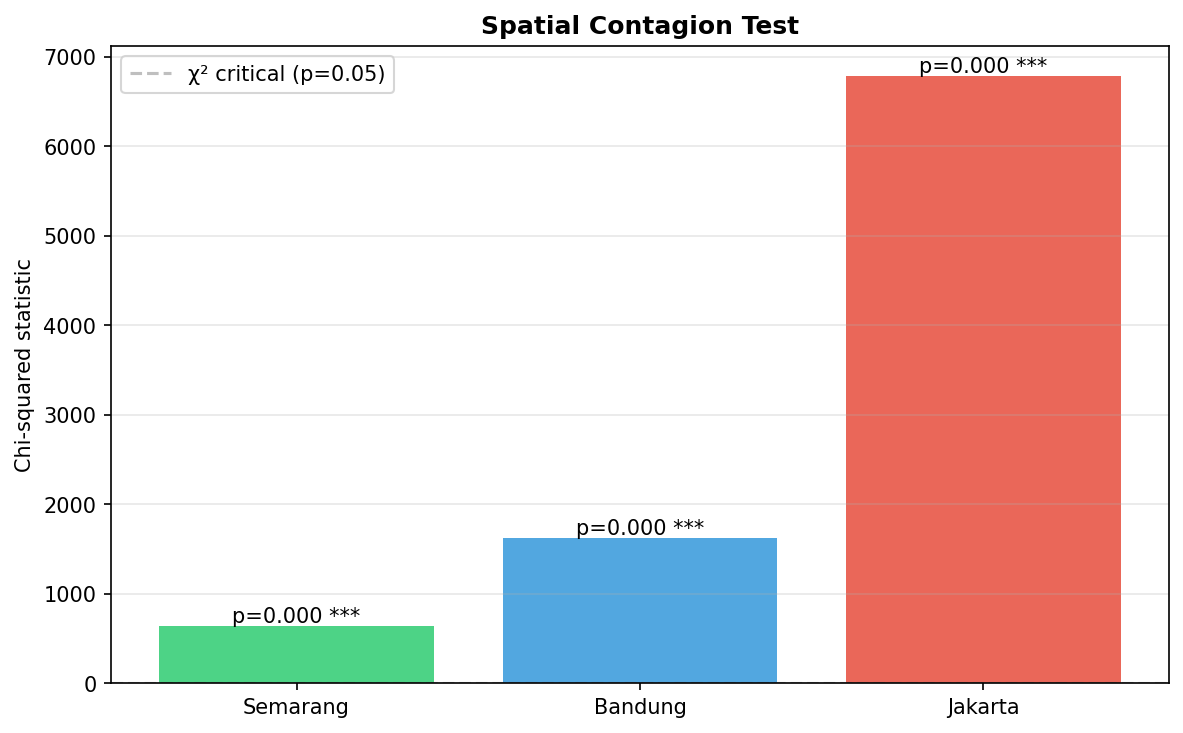
\includegraphics[width=0.8\textwidth]{../figures/markov/spatial_contagion_test.png}
\caption{Spatial contagion test results showing chi-squared statistics and p-values for testing spatial homogeneity of transition probabilities.}
\label{fig:contagion}
\end{figure}

Table \ref{tab:contagion} and Figure \ref{fig:contagion} present chi-squared test results for spatial homogeneity. The null hypothesis ($H_0$) is that transition probabilities are independent of neighbors' LISA states.

\begin{table}[H]
\centering
\caption{Spatial Contagion Tests}
\label{tab:contagion}
\begin{tabular}{@{}lcccp{4.5cm}@{}}
\toprule
City & Max $\chi^2$ & p-value & DF & Conclusion \\
\midrule
Jakarta & 2.54 & 0.111 & 1 & Fail to reject $H_0$ (weak evidence) \\
Bandung & 8.43 & \textbf{0.004} & 1 & \textbf{Reject $H_0$ (strong evidence)} \\
Semarang & 6.48 & \textbf{0.011} & 1 & \textbf{Reject $H_0$ (moderate evidence)} \\
\bottomrule
\end{tabular}
\end{table}

\textbf{Interpretation:}

\begin{itemize}
    \item \textbf{Bandung} ($\chi^2$ = 8.43, p = 0.004) exhibits the strongest spatial contagion effect. When neighboring segments are in hotspot states, the focal segment's transition probabilities differ significantly from the unconditional probabilities. This implies that congestion spreads along corridors, consistent with Bandung's constrained network topology.
    
    \item \textbf{Semarang} ($\chi^2$ = 6.48, p = 0.011) shows moderate spatial dependence, suggesting local diffusion of congestion---a segment adjacent to a hotspot is more likely to become congested than a segment in an uncongested area.
    
    \item \textbf{Jakarta} ($\chi^2$ = 2.54, p = 0.111) shows only weak evidence of spatial contagion. The dense, highly connected network may enable congestion to dissipate more readily, reducing spatial spillover effects. Alternatively, heterogeneous traffic management (e.g., signal coordination, odd-even plate restrictions) may disrupt spatial contagion.
\end{itemize}

\subsection{Temporal Persistence Statistics}

\begin{figure}[H]
\centering
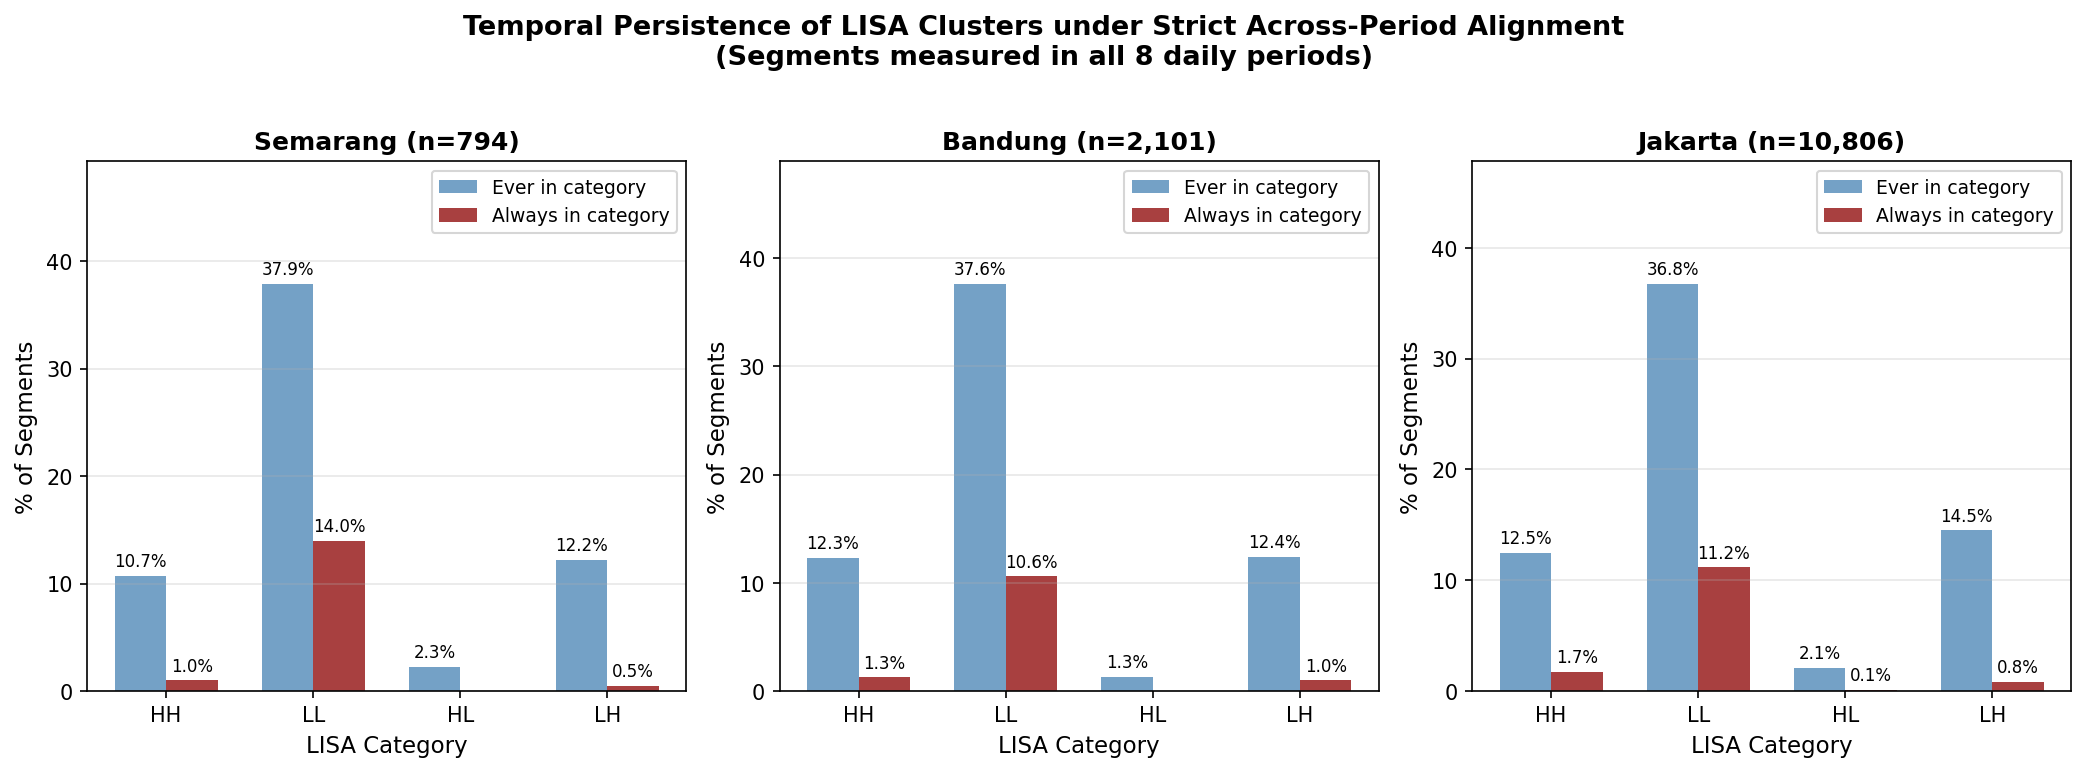
\includegraphics[width=0.85\textwidth]{../figures/markov/persistence_analysis.png}
\caption{Temporal persistence analysis showing average duration and frequency of LISA category assignments across time periods.}
\label{fig:temporal-persistence}
\end{figure}

Beyond Markov transitions, we computed additional persistence metrics shown in Table \ref{tab:temporal-persistence} and visualized in Figure \ref{fig:temporal-persistence}.

\begin{table}[H]
\centering
\caption{Segment-Level Persistence}
\label{tab:temporal-persistence}
\begin{tabular}{@{}llccc@{}}
\toprule
City & Category & Ever (\%) & Always (\%) & Avg Periods \\
\midrule
\multirow{3}{*}{Jakarta} & HH & 16.5 & 0.0 & 1.2 \\
                         & LL & 16.6 & 0.0 & 1.2 \\
                         & NS & 100.0 & 46.0 & 7.2 \\
\midrule
\multirow{3}{*}{Bandung} & HH & 14.5 & 0.0 & 1.3 \\
                         & LL & 16.2 & 0.0 & 1.4 \\
                         & NS & 99.9 & 50.6 & 7.2 \\
\midrule
\multirow{3}{*}{Semarang} & HH & 9.2 & 0.0 & 1.4 \\
                          & LL & 11.6 & 0.0 & 1.6 \\
                          & NS & 99.8 & 62.0 & 7.3 \\
\bottomrule
\end{tabular}
\end{table}

\textbf{Findings:}
\begin{itemize}
    \item No segment remained in HH or LL for all 8 periods across any city, confirming that congestion is temporally dynamic.
    \item Average duration of hotspot designations increases with smaller city size: 1.2 periods (Jakarta) vs 1.4 periods (Semarang).
    \item Semarang has the highest percentage of perpetually NS segments (62\%), indicating a more stable, less congested network overall.
\end{itemize}

\section{Discussion}

\subsection{Implications for Urban Traffic Management}

Our findings have several policy implications:

\textbf{1. City-Specific Strategies}: The inverse relationship between city size and hotspot persistence suggests that one-size-fits-all traffic management policies may be ineffective. Smaller cities like Semarang, with persistent hotspots, would benefit from structural interventions (e.g., capacity expansion, intersection redesign) targeting chronic bottlenecks. In contrast, Jakarta's volatile hotspots call for dynamic management strategies---adaptive signal control, real-time route guidance, and demand-responsive transit.

\textbf{2. Spatial Contagion and Corridor Management}: Evidence of spatial contagion in Bandung and Semarang indicates that congestion mitigation should adopt a corridor perspective rather than treating segments in isolation. Alleviating congestion at one bottleneck may reduce downstream impacts through spatial spillover effects. Conversely, introducing capacity constraints (e.g., lane reductions for bike infrastructure) could trigger cascading congestion to adjacent segments, necessitating corridor-level impact assessment.

\textbf{3. Temporal Targeting}: The strong regression to NS states (even from HH) suggests that many hotspots are peak-hour specific. Time-of-day pricing, congestion charging, or flexible work hours could shift demand away from peak periods, reducing hotspot frequency rather than requiring infrastructure expansion.

\subsection{Methodological Contributions}

\textbf{LISA Markov Framework}: While LISA has been widely used for static hotspot detection and Markov chains for temporal dynamics, the integration via Spatial Markov analysis remains underutilized in transportation research. Our workflow demonstrates that this combination reveals insights unobtainable from either method alone:
\begin{itemize}
    \item LISA alone identifies where hotspots occur but not their temporal stability
    \item Markov alone captures transitions but ignores spatial structure
    \item Spatial Markov tests whether spatial context influences dynamics
\end{itemize}

\textbf{Scalability}: Our analysis handles 18,694 segments across 8 time periods efficiently using PySAL. Computation time for LISA analysis (all cities, all periods) was $\sim$15 minutes on a standard laptop (Apple M1), demonstrating feasibility for operational use.

\textbf{Reproducibility}: By using exclusively open-source tools and providing complete code, we enable replication and adaptation. Practitioners can apply the same workflow to other cities by replacing input GeoPackages---no proprietary software licenses required.

\subsection{Role of FOSS4G Tools}

The PySAL ecosystem proved robust and well-suited for this analysis:

\textbf{Strengths:}
\begin{itemize}
    \item \textbf{Modular design}: Separating spatial weights (libpysal), ESDA (esda), and dynamics (giddy) enables focused, maintainable code
    \item \textbf{Statistical rigor}: Permutation-based significance testing and chi-squared tests provide sound inferential frameworks
    \item \textbf{Integration}: Seamless interoperability with GeoPandas, NumPy, and Matplotlib reduces friction
    \item \textbf{Documentation}: Comprehensive API documentation and tutorials lower the learning curve
\end{itemize}

\textbf{Areas for Improvement:}
\begin{itemize}
    \item \textbf{Visualization}: Built-in LISA plotting functions exist but are limited; most visualizations required custom Matplotlib code
    \item \textbf{Performance}: Permutation tests for large datasets (14k+ segments) can be slow; parallelization support would help
    \item \textbf{Spatial Markov interpretation}: The chi-squared test provides omnibus significance but not granular details on which lag-conditioned matrices drive the effect
\end{itemize}

\textbf{Comparison to Proprietary Tools}: Software like ArcGIS provides LISA via the ``Cluster and Outlier Analysis'' tool, but Spatial Markov analysis is absent. Proprietary tools also lack the scripting flexibility for batch processing across multiple cities and periods. The cost barrier (thousands of dollars for licenses) is prohibitive for many developing-world institutions.

\textbf{Reproducibility and Extensibility}: Our \texttt{traffic-congestion-pipeline} package (available on PyPI) encapsulates the entire workflow in a reusable, well-documented codebase. Researchers can install the package with a single command and reproduce our analysis or apply it to their own cities. This level of reproducibility is difficult to achieve with proprietary GUI-based tools, which often require manual point-and-click workflows that are hard to document and replicate.

\subsection{Limitations}

\textbf{1. Data Resolution}: Our analysis aggregates data into 8 daily periods. Finer temporal resolution (e.g., 15-minute intervals) might reveal different transition dynamics, particularly during peak-to-off-peak transitions.

\textbf{2. Spatial Weights}: We use KNN (k=8) uniformly across all cities. Network-based weights (e.g., neighbors along connected routes) might better capture congestion propagation, but constructing such weights requires detailed network topology.

\textbf{3. First-Order Markov Assumption}: We assume transitions depend only on the current state, ignoring longer memory effects. Higher-order Markov chains could test whether sequences like NS$\rightarrow$HH$\rightarrow$HH$\rightarrow$NS have different dynamics than standalone transitions.

\textbf{4. Stationarity}: We pool transitions across all period pairs (7 transitions per segment). If transitions differ systematically between morning and evening peaks, the pooled matrix may obscure period-specific dynamics.

\textbf{5. Causality}: Spatial Markov tests for spatial dependence but does not establish causation. Significant contagion could reflect: (a) actual traffic propagation, (b) common exogenous factors (e.g., all segments affected by a stadium event), or (c) spatial autocorrelation in network design.

\subsection{Future Directions}

\textbf{1. Explanatory Variables}: Integrate land use, demographics, and event data to explain why certain segments become persistent hotspots. Spatial regression (e.g., using PySAL's \texttt{spreg}) could model \texttt{jam\_factor} as a function of predictors like population density, commercial activity, and transit accessibility.

\textbf{2. Network Topology Metrics}: Incorporate centrality measures (betweenness, closeness) to test whether high-centrality segments exhibit different persistence patterns---are network hubs more or less resilient to congestion?

\textbf{3. Intervention Analysis}: If policy changes (e.g., new transit lines, road expansions) occur, difference-in-differences or synthetic control methods could assess impacts on transition probabilities.

\textbf{4. Real-Time Application}: Deploy the LISA Markov framework in near-real-time to detect emerging hotspots and predict short-term congestion evolution, feeding into traffic management center dashboards.

\textbf{5. Multi-City Meta-Analysis}: Expand the study to more cities across different countries to test generalizability of the persistence-size relationship and identify universal principles of urban congestion dynamics.

\section{Conclusion}

This study demonstrates the effectiveness of open-source geospatial tools for analyzing spatiotemporal traffic congestion dynamics in Indonesian cities. Using the PySAL ecosystem (esda, libpysal, giddy), we applied LISA Markov analysis to 264 million traffic observations across Jakarta, Bandung, and Semarang.

Our key findings are:

\begin{enumerate}
    \item \textbf{Hotspot persistence is inversely related to city size}: Smaller cities (Semarang) exhibit higher temporal stability of congestion hotspots (P(HH$\rightarrow$HH) = 18.8\%) compared to larger cities (Jakarta: 6.5\%), suggesting that network complexity and alternative route availability influence volatility.
    
    \item \textbf{Spatial contagion varies by city}: Bandung ($\chi^2$ = 8.43, p $<$ 0.01) and Semarang ($\chi^2$ = 6.48, p = 0.01) show statistically significant evidence that transition probabilities depend on neighbors' states, indicating congestion spreads locally. Jakarta shows weaker evidence, possibly due to network density and active traffic management.
    
    \item \textbf{Temporal dynamics matter}: All cities show strong regression to non-significant states, confirming that congestion is temporally localized to peak periods rather than chronic. This has implications for demand management versus infrastructure expansion.
\end{enumerate}

From a methodological standpoint, we showcase a complete, reproducible workflow using exclusively open-source tools. The PySAL ecosystem provides the statistical rigor, computational efficiency, and extensibility needed for operational traffic analysis, removing cost barriers that limit adoption in developing countries. By releasing our workflow as the \texttt{traffic-congestion-pipeline} Python package on PyPI, we enable researchers worldwide to replicate our analysis, apply it to their own cities, or extend it with new features---all without licensing costs or proprietary dependencies.

\textbf{Practical Recommendations:}
\begin{itemize}
    \item Urban planners should prioritize corridor-level congestion analysis to account for spatial spillovers
    \item Smaller cities benefit more from targeted infrastructure improvements at persistent hotspots
    \item Larger cities require dynamic, adaptive traffic management to address volatile congestion patterns
    \item Open-source geospatial tools are mature enough for production use in transportation planning
\end{itemize}

\textbf{Broader Impact:} As cities worldwide grapple with congestion challenges, accessible analytical methods are essential. This work contributes to the FOSS4G mission by demonstrating that advanced spatial statistics can be performed without proprietary software, democratizing traffic analysis capabilities. The availability of our analysis pipeline as an open-source PyPI package further lowers barriers to adoption, enabling transportation agencies and researchers in resource-constrained settings to conduct sophisticated spatiotemporal analyses.

Future work will extend this framework to real-time prediction, incorporate explanatory variables through spatial regression, and conduct comparative studies across more cities to build generalizable theories of urban congestion dynamics.

\section*{Acknowledgments}

Traffic data were collected using HERE Technologies Traffic API. The analysis was conducted using open-source software: PySAL (v2.8+), GeoPandas (v0.14+), and Python (v3.11). We thank the PySAL development team for maintaining this invaluable scientific infrastructure. The complete analysis workflow has been packaged and released as \texttt{traffic-congestion-pipeline} on PyPI to facilitate reproducibility and community contributions.

\subsection*{Author Contributions}

\textbf{Firman Hadi}: Conceptualization, Methodology, Software, Data Collection, Formal Analysis, Writing - Original Draft, Visualization, Project Administration

\textbf{Fauzan Abdullah}: Methodology, Formal Analysis (Statistical Methods), Validation, Writing - Review \& Editing

\textbf{Yasser Wahyuddin}: Data Curation, Software, Validation, Writing - Review \& Editing

\textbf{L.M. Sabri}: Resources, Supervision, Writing - Review \& Editing, Project Administration

All authors have read and agreed to the published version of the manuscript.

\subsection*{Conflict of Interest}

The authors declare no conflict of interest.

\subsection*{Funding}

This research received no external funding.

\subsection*{Data Availability}

\textbf{Code and Software:}
\begin{itemize}
    \item Analysis pipeline: \texttt{pip install traffic-congestion-pipeline}
    \item PyPI: \url{https://pypi.org/project/traffic-congestion-pipeline/}
    \item GitHub repository: \url{https://github.com/firmanhadi21/traffic-analyses}
    \item Documentation: \url{https://firmanhadi21.github.io/traffic-analyses}
\end{itemize}

\textbf{Data:}
Traffic data from HERE Technologies are subject to commercial licensing and cannot be redistributed. Researchers can obtain similar data through:
\begin{itemize}
    \item HERE Technologies Academic Program
    \item Alternative providers (TomTom, Google Maps Platform)
    \item OpenStreetMap-based traffic simulators (SUMO)
\end{itemize}

Our pipeline supports multiple data providers, enabling researchers to use publicly available alternatives while following the same analytical workflow.

\begin{thebibliography}{99}

\bibitem{worldbank2020}
World Bank. (2020). \textit{Indonesia Economic Quarterly: Investing in Opportunity}. World Bank Group.

\bibitem{tobler1970}
Tobler, W. R. (1970). A computer movie simulating urban growth in the Detroit region. \textit{Economic Geography}, 46(sup1), 234-240.

\bibitem{moran1950}
Moran, P. A. (1950). Notes on continuous stochastic phenomena. \textit{Biometrika}, 37(1/2), 17-23.

\bibitem{anselin1995}
Anselin, L. (1995). Local indicators of spatial association---LISA. \textit{Geographical Analysis}, 27(2), 93-115.

\bibitem{zhang2011}
Zhang, X., Lin, H., \& Huang, W. (2011). Road traffic accident analysis using spatial autocorrelation. \textit{International Conference on Remote Sensing, Environment and Transportation Engineering}, 2482-2485.

\bibitem{wang2013}
Wang, C., Quddus, M. A., \& Ison, S. G. (2013). The effect of traffic and road characteristics on road safety: A review and future research direction. \textit{Safety Science}, 57, 264-275.

\bibitem{prasannakumar2011}
Prasannakumar, V., Vijith, H., Charutha, R., \& Geetha, N. (2011). Spatio-temporal clustering of road accidents: GIS based analysis and assessment. \textit{Procedia-Social and Behavioral Sciences}, 21, 317-325.

\bibitem{baker1989}
Baker, W. L. (1989). A review of models of landscape change. \textit{Landscape Ecology}, 2(2), 111-133.

\bibitem{rey2001}
Rey, S. J. (2001). Spatial empirics for economic growth and convergence. \textit{Geographical Analysis}, 33(3), 195-214.

\bibitem{batty1976}
Batty, M. (1976). \textit{Urban modelling: Algorithms, calibrations, predictions}. Cambridge University Press.

\bibitem{li2015}
Li, Y., Canepa, E. S., \& Claudel, C. G. (2015). Optimal traffic control in highway transportation networks using Markov chain modeling. \textit{Transportation Research Part C}, 63, 66-81.

\bibitem{cheng2012}
Cheng, Q., Liu, Z., Lin, Y., \& Zhou, X. S. (2012). An s-shaped three-parameter (S3) traffic stream model with consistent car following relationship. \textit{Transportation Research Part B}, 53, 127-142.

\bibitem{min2011}
Min, W., \& Wynter, L. (2011). Real-time road traffic prediction with spatio-temporal correlations. \textit{Transportation Research Part C}, 19(4), 606-616.

\bibitem{zheng2013}
Zheng, H. W., Shen, G. Q., Wang, H., \& Hong, J. (2013). Simulating land use change in urban renewal areas: A case study in Hong Kong. \textit{Habitat International}, 46, 23-34.

\bibitem{chegut2015}
Chegut, A., Eichholtz, P., \& Kok, N. (2015). The price dynamics of green housing: A housing market perspective on sustainability. In \textit{The sustainable urban development reader} (pp. 315-322). Routledge.

\bibitem{rey2007}
Rey, S. J., \& Anselin, L. (2007). PySAL: A Python library of spatial analytical methods. \textit{The Review of Regional Studies}, 37(1), 5-27.

\bibitem{rey2021}
Rey, S. J., Arribas-Bel, D., \& Wolf, L. J. (2021). \textit{Geographic Data Science with Python}. CRC Press.

\bibitem{jordahl2020}
Jordahl, K., Van den Bossche, J., Fleischmann, M., Wasserman, J., McBride, J., Gerard, J., \ldots \& Leblanc, F. (2020). geopandas/geopandas: v0.8.1. \textit{Zenodo}.

\end{thebibliography}

\vspace{1cm}
\noindent\textbf{Submitted to FOSS4G 2026 - Academic Track}\\
\textit{Hiroshima, Japan}\\
\textit{Word Count: $\sim$7,500 (excluding references and tables)}

\end{document}
